\chapter{Design del sistema}

\section{Introduzione}
In questo documento mostreremo delle soluzioni concrete per il modello descritto nel documento di \docref{cha:analisi}, aggiungeremo quindi il \emph{come} al \emph{cosa}. Mostreremo quindi una specifica architetturale del sistema e aggiungeremo il necessario per rendere possibile l'implementazione dei requisiti formalizzati nel documento di \docref{cha:specifica_requisiti}.

\section{Architettura del sistema}
Vengono di seguito mostrate l'architettura fisica e quella software del sistema.

\subsection{Architettura fisica}
L'architettura fisica del sistema è mostrata dalla seguente figura:
\begin{center}
   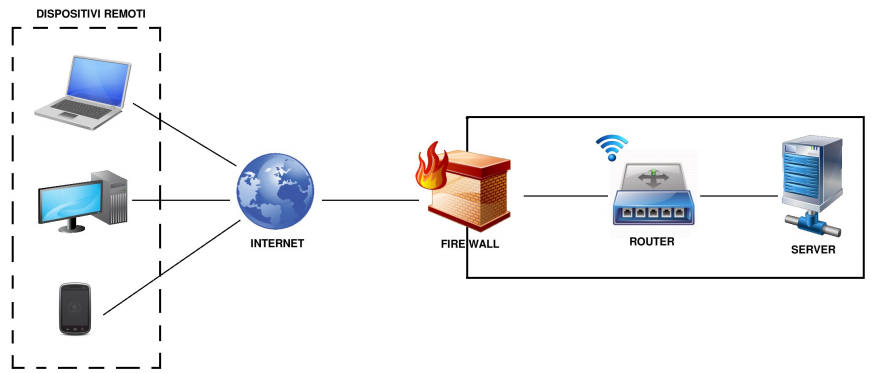
\includegraphics[width=\textwidth]{assets/architetturaFisica}
\end{center}

\subsection{Architettura software}
L'architettura software del sistema è mostrata dalla seguente figura:
\begin{center}
   \includegraphics[width=0.7\textwidth]{assets/architetturaSoftware}
\end{center}

\section{WordPress} \label{cms:wp}
Per realizzare il sistema finora descritto utilizzeremo il \gls{cms} commerciale WordPress, scelto in quanto dispone di una grande quantità di plugin per soddisfare tutte le funzionalità precedentemente descritte. Questo sarà installato nel server e si occuperà della comunicazione con i fruitori del servizio e integrerà il database.

\subsection{Installazione}
Per installare WordPress sarà necessario seguire i seguenti passi:
\begin{enumerate}
	\item Scaricare e decomprimere il pacchetto di WordPress;
	\item Creare un database per WordPress sul server web, ed un utente MySQL che abbia tutti i permessi per accederci e modificarlo;
	\item Rinominare il file \texttt{wp-config-sample.php} in \texttt{wp-config.php};
	\item Aprire \texttt{wp-config.php} in un editor di testo e inserire i dettagli del database;
	\item Caricare i file di WordPress nella cartella principale del server web;
	\item Lanciare lo script di installazione di WordPress visitando la pagina \texttt{http://esempio.com/wp-admin/install.php};
\end{enumerate}

\subsection{Configurazione}
Si dovranno creare le pagine descritte in fase di analisi, abilitare l'iscrizione ed il login al sito. Si dovranno inoltre installare, attivare e configurare tutti i plugin descritti nella prossima sezione.

\subsection{Plugin} \label{sec_plugin}
WordPress mette a disposizione oltre 47mila plugin, i quali estendono ed espandono le funzionalità di base presenti.
L'installazione e l'attivazione dei plugin è immediata, in quanto è possibile effettuarla direttamente tramite il pannello di controllo di WordPress.
Per implementare tutte le funzionalità precedentemente descritte sarà necessario installare ed attivare i seguenti plugin. Dovranno essere disattivate le funzioni fornite in eccesso dai plugin.

\subsubsection{User Role Editor} \label{plugin:ure}
\paragraph{Descrizione.} Con il plugin \gls{ure} è possibile cambiare le capacità di ogni ruolo. Basta spuntare le caselle di controllo delle capacità che si desidera aggiungere al ruolo selezionato. Aggiungere nuovi ruoli e personalizzarne le capacità in base alle proprie esigenze. Anche il ruolo assegnato di default alla creazione di ogni nuovo utente può essere modificato. Le capacità possono essere assegnate sulla base del singolo utente. Ruoli multipli possono essere assegnati all'utente simultaneamente. È possibile aggiungere nuove funzionalità e rimuovere le funzionalità non necessarie che potrebbero essere state lasciate da un plugin disinstallato.
\paragraph{Utilizzo.} \gls{ure} potrà essere utilizzato dall'amministratore per la gestione dei ruoli, dei profili, degli account e dell'assegnamento dei privilegi in base a quali ruoli un account possiede.
\paragraph{Configurazione.} Si dovranno creare i ruoli Visitatore, Utente, Produttore, Assistente, Redattore, Moderatore e Amministratore, assegnando ad ognuno i corrispettivi privilegi.

\subsubsection{Profile Builder Pro} \label{plugin:pbp}
\paragraph{Descrizione.} Il plugin \gls{pbp} permette di creare profili altamente personalizzabili. E' possibile inoltre creare e personalizzare form di iscrizione, login multipli. Permette di richiedere l'approvazione degli account a seconda del ruolo che assumono.
\paragraph{Utilizzo.}  \gls{pbp} potrà essere utilizzato per creare i profili utente e produttore, e approvare le richieste di iscrizione produttore. Potrà essere utilizzato per creare i form di registrazione per utenti e produttori.
\paragraph{Configurazione.}  Si dovranno creare i profili descritti e associarli agli account in base al loro ruolo. Si dovrà impostare l'iscrizione previa approvazione per le registrazioni di produttori. Si dovranno creare due form di registrazione: uno per gli utenti e i produttori.

\subsubsection{WooCommerce} \label{plugin:wc}
\paragraph{Descrizione.} \gls{wc} è un plugin per e-commerce gratuito che ti permette di vendere in maniera ottimale qualsiasi cosa. \gls{wc} fornisce sia ai proprietari che agli sviluppatori il controllo completo del proprio shop.
\paragraph{Utilizzo.} \gls{wc} potrà essere utilizzato per gestire la vetrina e l'inserimento e la modifica di prodotti, recensioni ad essi associate, commenti a recensioni, valutazioni e giudizi.
\paragraph{Configurazione.} Si dovrà configurare \gls{wc} in modo da non permettere la vendita di prodotti, ma solo la loro esposizione.
Per permettere a più produttori di avere la propria vetrina sarà necessaria l'installazione di \gls{wcv}.

\subsubsection{WC Vendors} \label{plugin:wcv}
\paragraph{Descrizione.} \gls{wcv} permette di creare il proprio marketplace e di fornire ai venditori la possibilità di vendere come su etsy, Envato, eBay, o Amazon. \gls{wcv} permette a più venditori di vendere i propri prodotti.
\paragraph{Utilizzo.} \gls{wcv} potrà essere utilizzato per gestire più vetrine contemporaneamente, permettendo ad ogni produttore di avere la propria vetrina in cui mostrare i propri prodotti.
\paragraph{Configurazione.} Non necessita di configurazione particolare.

\subsubsection{BuddyPress} \label{plugin:bp}
\paragraph{Descrizione.}
\gls{bp} è un insieme di componenti comuni a un tipico social network, e permette di aggiungere molte funzionalità attraverso l'esteso sistema di plugin di WordPress.
\gls{bp} è focalizzato sulla facilità di integrazione, facilità d'uso e estensibilità. È un software per creare social network volutamente potente anche se incredibilmente semplice, costruito dai contributori di WordPress.
\paragraph{Utilizzo.}
\gls{bp} potrà essere utilizzato per gestire il lato social del sistema, oltre a gestire le richieste dagli utenti ai produttori.
\paragraph{Configurazione.}
Per configurare \gls{bp} e gestire il sistema di follower/followed è necessario installare il plugin \gls{bpf}

\subsubsection{BuddyPress Follow} \label{plugin:bpf}
\paragraph{Descrizione.}
\gls{bpf} permette di estendere le funzionalità di \gls{bp} per implementare il sistema di follower/followed .
\paragraph{Utilizzo.} Verrà utilizzato per implementare il sistema di follower/followed.
\paragraph{Configurazione.} Non necessita di configurazione particolare.

\subsubsection{WP Support Plus Responsive Ticket System} \label{plugin:wpsprts}
\paragraph{Descrizione.} \gls{wpsprts} aggiunge a WordPress le funzionalità di un sistema di ticket completo. Permette alle persone autenticate di creare ticket per segnalare problemi o per ottenere supporto. I creatori del ticket possono impostare lo stato, la priorità e la categoria del ticket.
\paragraph{Utilizzo.} \gls{wpsprts} potrà essere utilizzato dalle persone autenticate per creare ticket per ottenere supporto.
\paragraph{Configurazione.} Non necessita di configurazione particolare.

\subsubsection{WP Report Post} \label{plugin:wprp}
\paragraph{Descrizione.} \gls{wprp} permette di segnalare post o pagine con contenuti inappropriati. Tutti questi report sono mostrati in una tabella nella sezione di Amministratore, permettendo così a quest'ultimo di scegliere cosa fare: modificare i contenuti, cancellare la pubblicazione di post/pagine, o semplicemente di eliminare i report. \gls{wprp} è progettato per funzionare sia in modo automatico che in modo manuale. In modo automatico, il link per segnalare potrà essere aggiunto al meta box del post. In modo manuale, si può aggiungere il link, il bottone o l'immagine dove si vuole nel template.
\paragraph{Utilizzo.} \gls{wprp} potrà essere utilizzato per inserire la possibilità di segnalare i contenuti del sistema, come schede prodotto, recensioni o commenti.
\paragraph{Configurazione.} Si dovrà configurare il link/bottone/immagine per effettuare la segnalazione su ogni contenuto segnalabile.

\subsubsection{Ninja Forms} \label{plugin:nf}
\paragraph{Descrizione.} \gls{nf} permette la creazione di form utilizzando un semplice drag-and-drop. Per i principianti è presente un design di creazione form semplice senza la necessità di scrivere codice. Gli sviluppatori, invece, possono utilizzare opzioni built-in, filtri, e template di campi personalizzati per la creazione di form di ogni tipo e anche per la loro sottomissione.
\paragraph{Utilizzo.} \gls{nf} potrà essere utilizzato per permettere la creazione dei form necessari all'interno del sistema, ad esempio per la Scheda Prodotto.
\paragraph{Configurazione.} Non necessita di configurazione particolare.

\subsubsection{Nextend Facebook Connect} \label{plugin:nfc}
\paragraph{Descrizione.} \gls{nfc} permette l'accesso tramite Facebook.
\paragraph{Utilizzo.} \gls{nfc} potrà essere utilizzato per permettere ai Visitatori di creare un account di tipo Utente utilizzando la funzinoalità di login tramite Facebook. Sarà perciò possibile effettuare il login con le credenziali di Facebook.
\paragraph{Configurazione.} Si dovrà configurare il bottone per effettuare il login tramite Facebook.

\subsubsection{SearchWP} \label{plugin:wps}
\paragraph{Descrizione.} \gls{wps} permette la personalizzazione della ricerca in diversi modi. E' possibile assegnare pesi ai diversi tipi di contenuti, cercare in base al tipo di contenuto o in base ai tag assegnati ai contenuti. Può essere esteso grazie alle molte estensioni disponibili e mette a disposizione diverse statistiche.
\paragraph{Utilizzo.} \gls{wps} potrà essere utilizzato per permettere la ricerca personalizzata in base alla tipologia di contenuto: Prodotto, Notizia o Profilo.
\paragraph{Configurazione.} Si dovrà configurare le ricerca personalizzata per Prodotti, Profili e Notizie. Inserire delle opzioni per selezionare quale tipo di ricerca effettuare.

\subsubsection{WP Related Post} \label{plugin:wprep}
\paragraph{Descrizione.} \gls{wprep} aggiunge in fondo alle pagine dei post visualizzati, i post all'interno del sito considerati simili. \gls{wprep} supporta differenti stili e miniature. E' completamente personalizzabile e include funzionalità di caching per migliorare le prestazioni.
\paragraph{Utilizzo.} \gls{wprep} potrà essere utilizzate per fornire suggerimenti di prodotti o notizie simili a quelle che si stanno visualizzando.
\paragraph{Configurazione.} Non necessita di configurazione particolare.

\subsubsection{Authy Two Factor Authentication} \label{plugin:atfa}
\paragraph{Descrizione.} \gls{atfa} aiuta ad incrementare la sicurezza degli account WordPress usando l'autenticazione a due passaggi. Ogni utente riceve un codice tramite sms, chiamata telefonica o tramite l'applicazione per smartphone Authy che dovrà inserire insieme alla sue credenziali. E' inoltre disponibile un sistema di notifiche push tramite l'applicazione Authy particolarmente sicuro. Permette di scegliere quali ruoli necessitano di autenticazione a due passaggi.
\paragraph{Utilizzo.} \gls{atfa} potrà essere utilizzato per permettere alle figure amministrative di effettuare l'autenticazione a due passaggi.
\paragraph{Configurazione.} Si dovranno impostare gli account amministrativi affinché sia richiesta l'autenticazione a due passaggi.

\subsection{Mapping classi di analisi}
In questa sezione mostreremo come questa configurazione del \gls{cms} implementa tutte le classi di analisi descritte nel documento di \docref{cha:analisi}. Va notato che non c'è una corrispondenza biunivoca fra un sottoinsieme delle classi e un sottoinsieme dei plugin, piuttosto diversi plugin possono servire a implementare una classe o, viceversa, più classi possono essere implementate da un singolo plugin.
Si noti che le scelte progettuali effettuate rendono agevole l'espansione del sistema con ulteriori funzionalità; inoltre i possibili problemi riscontrabili solo nella fase implementativa, come ad esempio la mancanza di alcune funzionalità necessarie per il corretto funzionamento del sistema, sono facilmente risolvibili installando ulteriori plugin. 
Di seguito vengono elencati i package e le classi di analisi definite nel documento di \docref{cha:analisi}:
\begin{itemize}
		\item \pkgCAT{pkg:Pagine}
		\begin{itemize}	
			\item \newListItem{classe:Pagina}{\formattaCLASSE}{Pagina} 
			\item \newListItem{classe:PaginaRecensione}{\formattaCLASSE}{PaginaRecensione} 
			\item \newListItem{classe:PaginaVetrina}{\formattaCLASSE}{PaginaVetrina} 
			\item \newListItem{classe:PaginaSegnalazioni}{\formattaCLASSE}{PaginaSegnalazioni} 
			\item \newListItem{classe:PaginaTicket}{\formattaCLASSE}{PaginaTicket} 
			\item \newListItem{classe:PaginaNotizie}{\formattaCLASSE}{PaginaNotizie} 
			\item \newListItem{classe:PaginaProfilo}{\formattaCLASSE}{PaginaProfilo} 
			\item \newListItem{classe:PaginaRichiesteIscrizioni}{\formattaCLASSE}{PaginaRichiesteIscrizioni} 
			\item \newListItem{classe:PaginaLogin}{\formattaCLASSE}{PaginaLogin} 
			\item \newListItem{classe:PaginaSchedaProdotto}{\formattaCLASSE}{PaginaSchedaProdotto} 			
			\item \newListItem{classe:PaginaAggiornamentiFollower}{\formattaCLASSE}{PaginaAggiornamentiFollower} 
			\item \newListItem{classe:PaginaRichiesteProdotto}{\formattaCLASSE}{PaginaRichiesteProdotto} 
			\item \newListItem{classe:PaginaIscrizione}{\formattaCLASSE}{PaginaIscrizione} 
			\item \newListItem{classe:Home}{\formattaCLASSE}{Home} 
		\end{itemize}	
		\item \pkgCAT{pkg:GestioneContenuti}
		\begin{itemize}	
			\item \newListItem{classe:GestioneSchedaProdotto}{\formattaCLASSE}{GestioneSchedaProdotto} 
			\item \newListItem{classe:GestioneNotizia}{\formattaCLASSE}{GestioneNotizia} 
			\item \newListItem{classe:GestioneRecensione}{\formattaCLASSE}{GestioneRecensione} 
		\end{itemize}	
		\item \pkgCAT{pkg:GestioneProfili}
		\begin{itemize}	
			\item \newListItem{classe:GestioneProfilo}{\formattaCLASSE}{GestioneProfilo} 
			\item \newListItem{classe:GestioneVetrina}{\formattaCLASSE}{GestioneVetrina} 
		\end{itemize}	
		\item \pkgCAT{pkg:GestioniComunicazioni}
		\begin{itemize}	
			\item \newListItem{classe:GestioneRichiesteProdotto}{\formattaCLASSE}{GestioneRichiesteProdotto} 
			\item \newListItem{classe:GestioneSegnalazioni}{\formattaCLASSE}{GestioneSegnalazioni} 
			\item \newListItem{classe:GestioneTicket}{\formattaCLASSE}{GestioneTicket} 
		\end{itemize}	
		\item \pkgCAT{pkg:GestioneSistema}
		\begin{itemize}	
			\item \newListItem{classe:GestioneAccessi}{\formattaCLASSE}{GestioneAccessi} 
			\item \newListItem{classe:GestioneIscritti}{\formattaCLASSE}{GestioneIscritti} 
			\item \newListItem{classe:Utility}{\formattaCLASSE}{Utility} 
			\item \newListItem{classe:Ricerca}{\formattaCLASSE}{Ricerca} 
		\end{itemize}	
		\item \pkgCAT{pkg:Contenuti}
		\begin{itemize}	
			\item \newListItem{classe:Contenuto}{\formattaCLASSE}{Contenuto} 
			\item \newListItem{classe:Commento}{\formattaCLASSE}{Commento} 
			\item \newListItem{classe:Recensione}{\formattaCLASSE}{Recensione} 
			\item \newListItem{classe:Giudizio}{\formattaCLASSE}{Giudizio} 
			\item \newListItem{classe:SchedaProdotto}{\formattaCLASSE}{SchedaProdotto} 
			\item \newListItem{classe:Valutazione}{\formattaCLASSE}{Valutazione} 
			\item \newListItem{classe:Notizia}{\formattaCLASSE}{Notizia} 
			\item \newListItem{classe:ConsistenzaProdotto}{\formattaCLASSE}{ConsistenzaProdotto} 
			\item \newListItem{classe:CategoriaProdotto}{\formattaCLASSE}{CategoriaProdotto} 
		\end{itemize}	
		\item \pkgCAT{pkg:Comunicazioni}
		\begin{itemize}	
			\item \newListItem{classe:Ticket}{\formattaCLASSE}{Ticket} 
			\item \newListItem{classe:RichiestaProduttore}{\formattaCLASSE}{RichiestaProduttore} 
			\item \newListItem{classe:RispostaTicket}{\formattaCLASSE}{RispostaTicket} 
			\item \newListItem{classe:RichiestaProdotto}{\formattaCLASSE}{RichiestaProdotto} 
			\item \newListItem{classe:SegnalazioneContenuto}{\formattaCLASSE}{SegnalazioneContenuto} 
		\end{itemize}	
		\item \pkgCAT{pkg:Iscrizioni}
		\begin{itemize}	
			\item \newListItem{classe:Account}{\formattaCLASSE}{Account} 
			\item \newListItem{classe:TipoAccount}{\formattaCLASSE}{TipoAccount} 
			\item \newListItem{classe:RichiestaIscrizione}{\formattaCLASSE}{RichiestaIscrizione} 
			\item \newListItem{classe:Privilegi}{\formattaCLASSE}{Privilegi} 
		\end{itemize}	
		\item \pkgCAT{pkg:Profili}
		\begin{itemize}	
			\item \newListItem{classe:Profilo}{\formattaCLASSE}{Profilo} 
			\item \newListItem{classe:ProfiloProduttore}{\formattaCLASSE}{ProfiloProduttore} 
			\item \newListItem{classe:Vetrina}{\formattaCLASSE}{Vetrina} 
		\end{itemize}	
		\item \pkgCAT{pkg:Autenticazione}
		\begin{itemize}	
			\item \newListItem{classe:AccessoIscritto}{\formattaCLASSE}{AccessoIscritto} 
			\item \newListItem{classe:AccessoOspite}{\formattaCLASSE}{AccessoOspite} 
		\end{itemize}	
		\item \pkgCAT{pkg:Utility}
		\begin{itemize}	
			\item \newListItem{classe:TipoRicerca}{\formattaCLASSE}{TipoRicerca} 
		\end{itemize}	
\end{itemize}
Nelle seguenti tabelle riportiamo il mapping effettuato fra le classi di analisi e il \gls{cms} con i suoi plugin che implementano quelle classi, in modo più strutturato rispetto a quanto già fatto nella sezione \docref{sec_plugin}:
\classeTab{classe:Pagina}
{\nameref{cms:wp}}
{\nameref{cms:wp} gestisce senza necessità di particolari plugin la creazione di pagine semplici}

\vspaceTab

\classeTab{classe:PaginaRecensione}
{\nameref{cms:wp}, \nameref{plugin:wc}}
{\nameref{cms:wp} gestisce la creazione delle pagine contenenti recensioni, mentre il plugin \nameref{plugin:wc} gestisce la visualizzazione delle recensioni}

\vspaceTab

\classeTab{classe:PaginaVetrina}
{\nameref{cms:wp}, \nameref{plugin:wc}, \nameref{plugin:wcv}}
{\nameref{cms:wp} gestisce la creazione delle pagine vetrina, il plugin \nameref{plugin:wc} gestisce la visualizzazione delle vetrine mentre il plugin \nameref{plugin:wcv} permette di avere negozi multipli (una vetrina per ogni produttore presente)}

\vspaceTab

\classeTab{classe:PaginaSegnalazioni}
{\nameref{cms:wp}, \nameref{plugin:wprp}}
{\nameref{cms:wp} gestisce la creazione delle pagine contenenti segnalazioni, mentre \nameref{plugin:wprp} gestisce l'intero sistema di segnalazioni con relativa visualizzazione da parte di un moderatore delle stesse}

\vspaceTab

\classeTab{classe:PaginaTicket}
{\nameref{cms:wp}, \nameref{plugin:wpsprts}}
{\nameref{cms:wp} gestisce la creazione delle pagine contenenti ticket, mentre \nameref{plugin:wpsprts} gestisce l'intero sistema di ticket con relativa visualizzazione da parte di un assistente delle stesse}

\vspaceTab

\classeTab{classe:PaginaNotizie}
{\nameref{cms:wp}, \nameref{plugin:wprep}}
{\nameref{cms:wp} gestisce senza necessità di particolari plugin la creazione di pagine contenenti notizie, \nameref{plugin:wprep} permette di visualizzare suggerimenti di notizie simili a quella mostrata}

\vspaceTab

\classeTab{classe:PaginaProfilo}
{\nameref{cms:wp}, \nameref{plugin:pbp}}
{\nameref{cms:wp} gestisce la creazione delle pagine profilo, \nameref{plugin:pbp} permette agli amministratori di creare profili personalizzati in base al tipo di account}

\vspaceTab 

\classeTab{classe:PaginaRichiesteIscrizioni}
{\nameref{cms:wp}, \nameref{plugin:pbp}}
{\nameref{cms:wp} gestisce la creazione delle pagine contenenti le richieste di iscrizione, \nameref{plugin:pbp} permette agli assistenti di visualizzare le richieste d'iscrizione delle persone che si iscrivono tramite il form d'iscrizione produttori}

\vspaceTab

\classeTab{classe:PaginaLogin}
{\nameref{cms:wp}, \nameref{plugin:nfc}}
{\nameref{cms:wp} gestisce la creazione della pagina di Login, \nameref{plugin:nfc} permette l'accesso tramite Facebook}

\vspaceTab

\classeTab{classe:PaginaSchedaProdotto}
{\nameref{cms:wp}, \nameref{plugin:wc}, \nameref{plugin:wcv}, \nameref{plugin:nf}, \nameref{plugin:wprep}}
{\nameref{cms:wp} gestisce la creazione delle pagine prodotto, \nameref{plugin:wc} e \nameref{plugin:wcv} permettono ai produttori di mostrare i propri prodotti, \nameref{plugin:nf} permette di personalizzare i campi della scheda prodotto, \nameref{plugin:wprep} permette di visualizzare suggerimenti di prodotti simili a quello mostrato}

\vspaceTab

\classeTab{classe:PaginaAggiornamentiFollower}
{\nameref{cms:wp}, \nameref{plugin:bp}, \nameref{plugin:bpf}}
{\nameref{cms:wp} gestisce la creazione delle pagine in cui si possono visualizzare gli aggiornamenti delle persone che si seguono, \nameref{plugin:bp} esteso con \nameref{plugin:bpf} implementa le funzionalità di follower/followed}

\vspaceTab

\classeTab{classe:PaginaRichiesteProdotto}
{\nameref{cms:wp}, \nameref{plugin:bp}, \nameref{plugin:nf}}
{\nameref{cms:wp} gestisce la creazione delle pagine contenenti le richieste prodotto, \nameref{plugin:bp} permette di visualizzare le richieste prodotto ricevute, \nameref{plugin:nf} permette la gestione dei form delle richieste prodotto}

\vspaceTab

\classeTab{classe:PaginaIscrizione}
{\nameref{cms:wp}, \nameref{plugin:pbp}, \nameref{plugin:nfc}}
{\nameref{cms:wp} gestisce la creazione delle pagine di iscrizione, \nameref{plugin:pbp} permette di creare form di iscrizione multipli, quindi un form per l'iscrizione di account che otterrano ruolo utente e uno per quelli che otterrano ruolo produttore, \nameref{plugin:nfc} permette di effettuare l'iscrizione direttamente con le credenziali di Facebook (effettuando direttamente il login)}

\vspaceTab

\classeTab{classe:Home}
{\nameref{cms:wp}, \nameref{plugin:wc}, \nameref{plugin:wps}}
{\nameref{cms:wp} gestisce la creazione della pagina home, \nameref{plugin:wc} permette di cercare i contenuti inseriti, \nameref{plugin:wps} permette di personalizzare la metodologia di ricerca, in particolare permette di ricercare: solo prodotti, solo profili o solo notizie}

\vspaceTab

\classeTab{classe:GestioneSchedaProdotto}
{\nameref{plugin:wc}, \nameref{plugin:wcv}, \nameref{plugin:wprep}}
{\nameref{plugin:wc} e \nameref{plugin:wcv} permettono ad ogni Produttore di gestire le proprie schede prodotto (inserire/modificare), \nameref{plugin:wprep} permette di ricevere suggerimenti di prodotti simili a quello mostrato}

\vspaceTab

\classeTab{classe:GestioneNotizia}
{\nameref{cms:wp}, \nameref{plugin:wprep}}
{\nameref{cms:wp} gestisce senza necessità di particolari plugin la creazione di pagine contenenti notizie, \nameref{plugin:wprep} permette di ricevere suggerimenti di notizie simili a quella mostrata}

\vspaceTab

\classeTab{classe:GestioneRecensione}
{\nameref{plugin:wc}, \nameref{plugin:wcv}}
{\nameref{plugin:wc} e \nameref{plugin:wcv} permettono di gestire il sistema di recensioni dei prodotti}

\vspaceTab

\classeTab{classe:GestioneProfilo}
{\nameref{cms:wp}, \nameref{plugin:pbp}, \nameref{plugin:bp}, \nameref{plugin:bpf}}
{\nameref{cms:wp} permette la gestione del profilo, \nameref{plugin:pbp} permette agli amministratori di creare profili personalizzati in base al tipo di account, \nameref{plugin:bp} e \nameref{plugin:bpf} permettono di gestire le funzionalità di follower/followed}

\vspaceTab

\classeTab{classe:GestioneVetrina}
{\nameref{plugin:wc}, \nameref{plugin:wcv}}
{\nameref{plugin:wc} esteso tramite il plugin \nameref{plugin:wcv} permettono ai produttori di avere una loro vetrina, contenente i loro prodotti}

\vspaceTab

\classeTab{classe:GestioneRichiesteProdotto}
{\nameref{plugin:bp}, \nameref{plugin:nf}}
{\nameref{plugin:bp} permette la comunicazione fra gli utenti, \nameref{plugin:nf} permette la gestione dei form delle richieste prodotto all'interno delle comunicazioni}


\vspaceTab

\classeTab{classe:GestioneSegnalazioni}
{\nameref{cms:wp}, \nameref{plugin:wprp}}
{\nameref{cms:wp} permette di gestire le segnalazioni, mentre \nameref{plugin:wprp} gestisce l'intero sistema di segnalazioni con relativa visualizzazione da parte di un moderatore delle stesse}

\vspaceTab

\classeTab{classe:GestioneTicket}
{\nameref{plugin:wpsprts}}
{\nameref{plugin:wpsprts} gestisce l'intero sistema di ticket con relativa visualizzazione da parte di un assistente delle stesse}

\vspaceTab

\classeTab{classe:GestioneAccessi}
{\nameref{cms:wp}, \nameref{plugin:ncf}, \nameref{plugin:atfa}}
{\nameref{cms:wp} permette di gestire gli accessi al sistema da parte di iscritti e di visitatori, \nameref{plugin:ncf} permette l'accesso tramite Facebook, \nameref{plugin:atfa} abilita l'autenticazione a due passaggi per le figure amministrative}

\vspaceTab

\classeTab{classe:GestioneIscritti}
{\nameref{cms:wp}, \nameref{plugin:pbp}, \nameref{plugin:ure}}
{\nameref{cms:wp} mette a diposizione la gestione base dell'iscrizione e degli account iscritti,  \nameref{plugin:pbp} permette di creare due diverse procedure di iscrizione: per i produttori e per gli utenti. Inoltre permette di accettare le iscrizioni dei produttori solo previa approvazione, \nameref{plugin:ure} permette la gestione dei tipi di un account}

\vspaceTab

\classeTab{classe:Utility}
{\nameref{cms:wp}}
{\nameref{cms:wp} permette l'estensione di funzionalità tramite l'utilizzo di plugin}

\vspaceTab

\classeTab{classe:Ricerca}
{\nameref{plugin:wc}, \nameref{plugin:wps}}
{\nameref{plugin:wc} permette di cercare i contenuti inseriti, \nameref{plugin:wps} permette di personalizzare la metodologia di ricerca, in particolare permette di ricercare: solo prodotti, solo profili o solo notizie}

\vspaceTab

\classeTab{classe:Contenuto}
{\nameref{plugin:wc}}
{\nameref{plugin:wc} permette la creazione di contenuti come schede prodotto, recensioni, commenti, valutazioni o giudizi}

\vspaceTab

\classeTab{classe:Commento}
{\nameref{plugin:wc}}
{\nameref{plugin:wc} permette di creare commenti a recensioni}

\vspaceTab

\classeTab{classe:Recensione}
{\nameref{plugin:wc}}
{\nameref{plugin:wc} permette di creare recensioni di prodotti}

\vspaceTab

\classeTab{classe:Giudizio}
{\nameref{plugin:wc}}
{\nameref{plugin:wc} permette di inserire giudizi per commenti}

\vspaceTab

\classeTab{classe:SchedaProdotto}
{\nameref{plugin:wc}, \nameref{plugin:nf}}
{\nameref{plugin:wc} e \nameref{plugin:nf} permettono di creare schede prodotti con i campi necessari}

\vspaceTab

\classeTab{classe:Valutazione}
{\nameref{plugin:wc}}
{\nameref{plugin:wc} permette di inserire valutazioni per recensioni}

\vspaceTab

\classeTab{classe:Notizia}
{\nameref{cms:wp}}
{\nameref{cms:wp} permette di creare post contenenti notizie}

\vspaceTab

\classeTab{classe:ConsistenzaProdotto}
{\nameref{plugin:nf}}
{\nameref{plugin:nf} permette di creare campi a scelta multipla}

\vspaceTab

\classeTab{classe:CategoriaProdotto}
{\nameref{plugin:nf}}
{\nameref{plugin:nf} permette di creare campi a scelta multipla}

\vspaceTab

\classeTab{classe:Ticket}
{\nameref{plugin:wpsprts}}
{\nameref{plugin:wpsprts} permette la creazione di ticket per richiedere assistenza}

\vspaceTab

\classeTab{classe:RichiestaProduttore}
{\nameref{plugin:wpsprts}}
{\nameref{plugin:wpsprts} permette la creazione di richieste produttore, creando tipologie di ticket personalizzate}

\vspaceTab

\classeTab{classe:RispostaTicket}
{\nameref{plugin:wpsprts}}
{\nameref{plugin:wpsprts} permette la creazione di risposte ad un ticket}

\vspaceTab

\classeTab{classe:RichiestaProdotto}
{\nameref{plugin:bp}, \nameref{plugin:nf}}
{\nameref{plugin:bp} e \nameref{plugin:nf} permettono l'invio di richieste prodotto ai produttori, attraverso l'utilizzo di messaggi strutturati con un form integrato}

\vspaceTab

\classeTab{classe:SegnalazioneContenuto}
{\nameref{plugin:wprp}}
{\nameref{plugin:wprp} permette di creare segnalazioni di contenuti all'interno del sistema}

\vspaceTab

\classeTab{classe:Account}
{\nameref{cms:wp}, \nameref{plugin:pbp}, \nameref{plugin:ure}, \nameref{plugin:nfc}}
{\nameref{cms:wp} permette di gestire gli account iscritti senza estenzioni, \nameref{plugin:pbp} permette di modificare le informazioni inserite in fase di registrazione (anche in base al ruolo che si vuole ottenre, Utene o Produttore), e quindi modificare le informazioni note dell'account, \nameref{plugin:ure} permette di modificare i ruoli degli account, fornendogli di conseguenza le funzionalità associate, \nameref{plugin:nfc} gestisce gli account iscritti tramite Facebook}

\vspaceTab

\classeTab{classe:TipoAccount}
{\nameref{plugin:ure}}
{\nameref{plugin:ure} permette la creazione di diversi ruoli (nell'analisi chiamati TipoAccount) a cui associare diverse funzionalità (nell'analisi chiamate privilegi)}

\vspaceTab

\classeTab{classe:RichiestaIscrizione}
{\nameref{plugin:pbp}}
{\nameref{plugin:pbp} permette la creazione di un form personalizzato per la registrazione dei produttori, ai quali verrà permessa l'iscrizione solo previa approvazione da parte dell'assistente}

\vspaceTab

\classeTab{classe:Privilegi}
{\nameref{cms:wp}}
{\nameref{cms:wp} gestisce l'inserimento di ogni funzionalità aggiunta tramite plugin. L'elenco delle funzionalità sarà perciò costituito da quelle di \nameref{cms:wp} estese da quelle dei plugin installati ed attivati}

\vspaceTab

\classeTab{classe:Profilo}
{\nameref{cms:wp}, \nameref{plugin:pbp}}
{\nameref{cms:wp} permette la modifica del profilo, \nameref{plugin:pbp} permette agli amministratori di creare profili personalizzati in base al tipo di account}

\vspaceTab

\classeTab{classe:ProfiloProduttore}
{\nameref{cms:wp}, \nameref{plugin:pbp}}
{\nameref{cms:wp} permette la modifica del profilo, \nameref{plugin:pbp} permette agli amministratori di creare profili personalizzati in base al tipo di account. In particolare i profili dei produttori avranno una vetrina associata}

\vspaceTab

\classeTab{classe:Vetrina}
{\nameref{plugin:wc}, \nameref{plugin:wcv}}
{\nameref{plugin:wc} gestisce la vetrine, creandone una alla creazione di ogni account produttore, mentre il plugin \nameref{plugin:wcv} permette di avere negozi multipli (una vetrina per ogni produttore presente)}

\vspaceTab

\classeTab{classe:AccessoIscritto}
{\nameref{cms:wp}}
{\nameref{cms:wp} il controllo degli accessi degli iscritti al sistema}

\vspaceTab

\classeTab{classe:AccessoOspite}
{\nameref{cms:wp}}
{\nameref{cms:wp} il controllo degli accessi dei visitatori al sistema}

\vspaceTab

\classeTab{classe:TipoRicerca}
{\nameref{plugin:wps}}
{\nameref{plugin:wps} permette la creazione di tipi di ricerca personalizzati}


\newdate{designuno}{24}{10}{2016}
\newdate{designdue}{25}{10}{2016}
\section{Revisioni}
\begin{center}
	\begin{tabular}
	{lll}
		\toprule
		\tabhead{Versione} & \tabhead{Data} & \tabhead{Descrizione} \\
		\cmidrule(l{\cmidrulekern}r{\cmidrulekern}){1-3}
		1.0 & \displaydate{designuno} & Prima versione \\        
		2.0 & \displaydate{designdue} & Aggiunto mapping \\        
		\bottomrule
	\end{tabular}
\end{center}
